\documentclass[usenames,dvipsnames]{beamer}

\mode<presentation> {

% The Beamer class comes with a number of default slide themes
% which change the colors and layouts of slides. Below this is a list
% of all the themes, uncomment each in turn to see what they look like.

%\usetheme{default}
% \usetheme{AnnArbor}
%\usetheme{Antibes}
%\usetheme{Bergen}
% \usetheme{Berkeley}
% \usetheme{Berlin}
%\usetheme{Boadilla}
%\usetheme{CambridgeUS}
% \usetheme{Copenhagen}
\usetheme{Darmstadt}
% \usetheme{Dresden}
% \usetheme{Frankfurt}
% \usetheme{Goettingen}
%\usetheme{Hannover}
%\usetheme{Ilmenau}
%\usetheme{JuanLesPins}
%\usetheme{Luebeck}
% \usetheme{Madrid}
% \usetheme{Malmoe}
%\usetheme{Marburg}
% \usetheme{Montpellier}
% \usetheme{PaloAlto}
% \usetheme{Pittsburgh}
%\usetheme{Rochester}
% \usetheme{Singapore}
%\usetheme{Szeged}
%\usetheme{Warsaw}

% As well as themes, the Beamer class has a number of color themes
% for any slide theme. Uncomment each of these in turn to see how it
% changes the colors of your current slide theme.

% \usecolortheme{albatross}
%\usecolortheme{beaver}
%\usecolortheme{beetle}
%\usecolortheme{crane}
%\usecolortheme{dolphin}
%\usecolortheme{dove}
%\usecolortheme{fly}
\usecolortheme{lily}
%\usecolortheme{orchid}
%\usecolortheme{rose}
%\usecolortheme{seagull}
%\usecolortheme{seahorse}
%\usecolortheme{whale}
%\usecolortheme{wolverine}

%\setbeamertemplate{footline} % To remove the footer line in all slides uncomment this line
%\setbeamertemplate{footline}[page number] % To replace the footer line in all slides with a simple slide count uncomment this line

\setbeamertemplate{navigation symbols}{} % To remove the navigation symbols from the bottom of all slides uncomment this line
}

% % -------------------------------------------
% % Songkai added, feel free to delete --------
% \AtBeginSection[]{
%   \begin{frame}
%   \vfill
%   \centering
%   \begin{beamercolorbox}[sep=8pt,center,shadow=false,rounded=true]{title}
%     \usebeamerfont{title}\insertsectionhead\par%
%   \end{beamercolorbox}
%   \vfill
%   \end{frame}
% }
% % Songkai added, feel free to delete --------
% % -------------------------------------------




\usepackage{graphicx} % Allows including images
\usepackage{booktabs} % Allows the use of \toprule, \midrule and \bottomrule in tables
\usepackage{natbib}
\usepackage{amsmath, amssymb, graphicx, url}
\usepackage[ruled]{algorithm2e}
\usepackage{commath}
\usefonttheme[onlymath]{serif}

\usepackage{amsmath}
\usepackage{amssymb}
\usepackage{centernot}
\usepackage{comment}
%\usepackage[a4paper, margin=0.8in]{geometry}
\usepackage{parskip}
\usepackage{graphicx}

\usepackage{natbib}

\usepackage{tikz}
\usepackage{tikzlings}

\usepackage{tabularx}
\usepackage{array}
\usepackage{multirow}
\usepackage{makecell}
\usepackage{mathtools}
\usepackage{bm,upgreek}
\usepackage{subcaption}
\usepackage{textpos}
% \usepackage{eso-pic}

% \usepackage{multimedia}
\usepackage{media9}

\def\E{\mathbf{E}}
\def\PP{\mathbf{P}}
\def\Reals{\mathbb{R}}
\def\Naturals{\mathbb{N}}
\def\argmin{\operatornamewithlimits{arg\,min}}
\def\deq{:=}
\def\wh#1{\widehat{#1}}
\def\bd#1{\mathbf{#1}}
\def\bx{\bd{x}}
\def\by{\bd{y}}
\def\bZ{\bd{Z}}
\def\bB{\bd{B}}
\def\bV{\bd{V}}
\def\tO{{\tilde{\cO}}}
\def\tOm{\tilde{\Omega}}
\def\barw{\overline{w}}
\def\d{{\mathrm d}}
\def\ave#1{\langle #1 \rangle}
\def\Ave#1{\left\langle #1 \right\rangle}
\def\eps{\varepsilon}
\def\tr{\mathrm{Tr}}


\def\HS{\mathbb{H}}
\def\reals{\mathbb{R}}
\def\ths{\theta^*}
\def\thh{\hat{\theta}}
\def\lbr{\left[}
\def\rbr{\right]}
\def\lc{\left(}
\def\rc{\right)}


    \def\ddefloop#1{\ifx\ddefloop#1\else\ddef{#1}\expandafter\ddefloop\fi}
    % \cA, \cB, ...
    \def\ddef#1{\expandafter\def\csname c#1\endcsname{\ensuremath{\mathcal{#1}}}}
    \ddefloop ABCDEFGHIJKLMNOPQRSTUVWXYZ\ddefloop
    \def\argmin{\operatornamewithlimits{arg\,min}}
    \def\E{\mathbf{E}}
    \def\bx{\bd{x}}
	\def\by{\bd{y}}
    \def\bZ{\bd{Z}}

\newcommand{\propnumber}{} % initialize
\newtheorem*{prop}{Proposition \propnumber}
\newenvironment{propc}[1]
  {\renewcommand{\propnumber}{#1}%
   \begin{shaded}\begin{prop}}
  {\end{prop}\end{shaded}}

\newcommand{\crlrnumber}{} % initialize
%\newtheorem*{corollary}{Corollary \crlrnumber}
\newenvironment{corollaryc}[1]
  {\renewcommand{\crlrnumber}{#1}%
   \begin{shaded}\begin{corollary}}
  {\end{corollary}\end{shaded}}

\theoremstyle{definition}
% \newtheorem{definition}




% \setbeamertemplate{headline}{% 
%     \leavevmode%
%     \hbox{%
%         \begin{beamercolorbox}[wd=.4\paperwidth,ht=2.25ex,dp=1ex,right]{section in head/foot}%
%             \usebeamerfont{section in head/foot}\insertshorttitle\hspace*{2ex}
%         \end{beamercolorbox}%
%         \begin{beamercolorbox}[wd=.6\paperwidth,ht=2.25ex,dp=1ex,left]{subsection in head/foot}%
%             \usebeamerfont{section in head/foot}
\includegraphics[height=2ex,keepaspectratio]{Slides/Block_M-Hex.png}\hspace*{2ex}\insertsectionhead
%         \end{beamercolorbox}%
%     }
% }

% \addtobeamertemplate{headline}{}{%
% \begin{textblock*}{100mm}(.85\textwidth,-1cm)
% \Huge\textcolor{white}{\textbf{\TeX}}
% \end{textblock*}}



%----------------------------------------------------------------------------------------
%	TITLE PAGE
%----------------------------------------------------------------------------------------

%%%% TRY WITH TEXTPOS
% \newcommand{\imgblock}{\begin{textblock*}{5cm}(10.5cm,-1.2cm) % {block width} (coords)
%         
\includegraphics[width=1cm]{Slides/Block_M-Hex.png} % loading the image
%     \end{textblock*}
%     }

% \addtobeamertemplate{background}{\imgblock}{}



% \setbeamertemplate{headline}{\hfill
\includegraphics[width=1.5cm]{Slides/Block_M-Hex.png}\hspace{0.2cm}\vspace{-1cm}}

% \logo{
\includegraphics[height=1cm]{Slides/Block_M-Hex.png}}

\addtobeamertemplate{frametitle}{}{%
    \begin{textblock*}{5cm}(10.5cm, -0.8cm)
        
\includegraphics[width=0.9cm]{Block_M-Hex.png} % your logo file here
    \end{textblock*}
}

\definecolor{mycolor}{cmyk}{100, 60, 0, 60}
\definecolor{my_maize}{rgb}{0.9608,0.7137,0.2588}
\definecolor{my_yellow}{rgb}{0.9294,0.8196,0.2706}

% \setbeamercolor{section in head/foot}{fg=cyan}
\setbeamercolor{section in head/foot}{fg=my_maize}

\setbeamercolor{frametitle}{bg=mycolor}
\setbeamercolor{titlelike}{fg=black, bg=yellow}

\usepackage{url}
\usepackage{hyperref}

\usepackage{xcolor}

\hypersetup{pdfauthor={Name},
            colorlinks=true,
            linkcolor={my_yellow},
            % citecolor={blue},
            % linkcolor=[RGB]{0.949, 0.784, 0.035}
            }

% fix inconsistent colors in cite parenthesis (where the closing parenthesis were black instead of the rest of the citecolor!)
% https://github.com/josephwright/beamer/issues/671
\let\oldcite=\cite
\let\oldcitet=\citet
\let\oldcitep=\citep 
\renewcommand{\citet}[2][]{\textcolor{green}{\oldcitet[#1]{#2}}}
\renewcommand{\citep}[2][]{\textcolor{green}{\oldcitep[#1]{#2}}}
\renewcommand{\cite}[2][]{\textcolor{green}{\oldcite[#1]{#2}}}
            

\title[Seminar]{Part 1 - A Useless Tutorial for using KG}
% \title[Seminar]{An Adaptive Bayesian Method for Covariance Estimation in Multifidelity Estimators}

% and Estimation of Predictive Uncertainties
% The short title appears at the bottom of every slide, the full title is only on the title page

\author[AJ]{Aniket}
\institute[U-M]{University of Michigan}

\date{22 Aug}

\AtBeginSection[]
{
 \begin{frame}<beamer>
 \frametitle{Plan}
 \tableofcontents[currentsection]
 \end{frame}
}


\begin{document}

\begin{frame}
\titlepage % Print the title page as the first slide
\end{frame}


% \begin{frame}{Notes}
% \end{frame}
\begin{frame}{Overview}

A presentation in multiple parts that:

\begin{enumerate}
    \item Adds to our toolbox of acquisition functions: UCB, PI, EI (Expected Improvement) with another acronym
    
    \item Sequential sampling policies with KG
    
    \item Applications (covariance emulation)
\end{enumerate}

\end{frame}


\begin{frame}{KG Definition}

\end{frame}

\begin{frame}{KG Definition}
    
\end{frame}

\begin{frame}{Acquisition and Updates}
    
\end{frame}

\begin{frame}{Acquisition and updates}


\end{frame}

\begin{frame}{Comparisons with EI}
    
\end{frame}

\begin{frame}{Preview for Part II}

\end{frame}

% \begin{frame}
%  \frametitle{Overview} % Table of contents slide, comment this block out to remove it
%  \tableofcontents % Throughout your presentation, if you choose to use \section{} and \subsection{} commands, these will automatically be printed on this slide as an overview of your presentation
% \end{frame}

% \section{Background}
% \begin{frame}{ODEs and PDEs}
% \textbf{Paper:} \cite{Chkrebtii2016}

% $$u: \mathcal{D} \times \Theta \to \mathbb{R}^p$$ satisfies a PDE for $(x, t) \in \mathcal{D} \cup \partial \mathcal{D}$:

% $$F(x, t, \partial_t u, \partial_{x_1} u, \cdots, u, \theta)=0$$

% Solution: $u^{\ast}(x, t)$ - generally not available in closed form.

% \textbf{Approximation:} $N$-dimensional: $\hat{u}^N(x, t, \theta)$ for size $N$ partitioning of domain $\mathcal{D}$

% \end{frame}

% \begin{frame}{Addressing Uncertainties}
% Commonly, forward UQ propagates of uncertainties from $\theta$ to $\hat{u}$

% \textbf{Verification}: \cite{roy_comprehensive_2011} - The characterization of the numerical approximation errors associated with a simulation. Includes:

% \begin{enumerate}
% \item Discretization error (usually the largest)
% \item Iterative convergence errors (equations resulting from discretization are solved approximately)
% \item Round off errors
% \end{enumerate}

% \textbf{Neglected: } \emph{Verification error} - Discretization errors are often ignored in practice. Introduces perturbations leading to exponential divergence from exact solution in \textcolor{red}{chaotic systems.}

% \emph{Costly} to maintain fine-enough mesh to ignore discretization-related issues.

% \end{frame}

% \begin{frame}{Objective of Paper}
%     \begin{enumerate}
%         \item Model discretization uncertainty through lens of Bayesian methods.
        
%         \item Develop probabilistic solution marginalized over model queries $f_n$ at grid locations.
        
%         \item Show application of methods as diagnostic tool for discretization effects in posterior under-coverage.
%     \end{enumerate}
% \end{frame}

% \begin{frame}{Related Work}
% \begin{enumerate}
%     \item \emph{Early work} - Bayesian solution for ODEs - \cite{Skilling1992}

%     \item Probabilistic Numerics \cite{hennig_probabilistic_2015} - highlight connections between `deterministic' numerical algorithms and probabilistic priors e.g. Quadrature rules as varying assumptions for GP parameters / kernel functions. \footnote[1]{follow up: recast ODEs as state estimation problems}
    
%     \begin{figure}
%         \centering
%         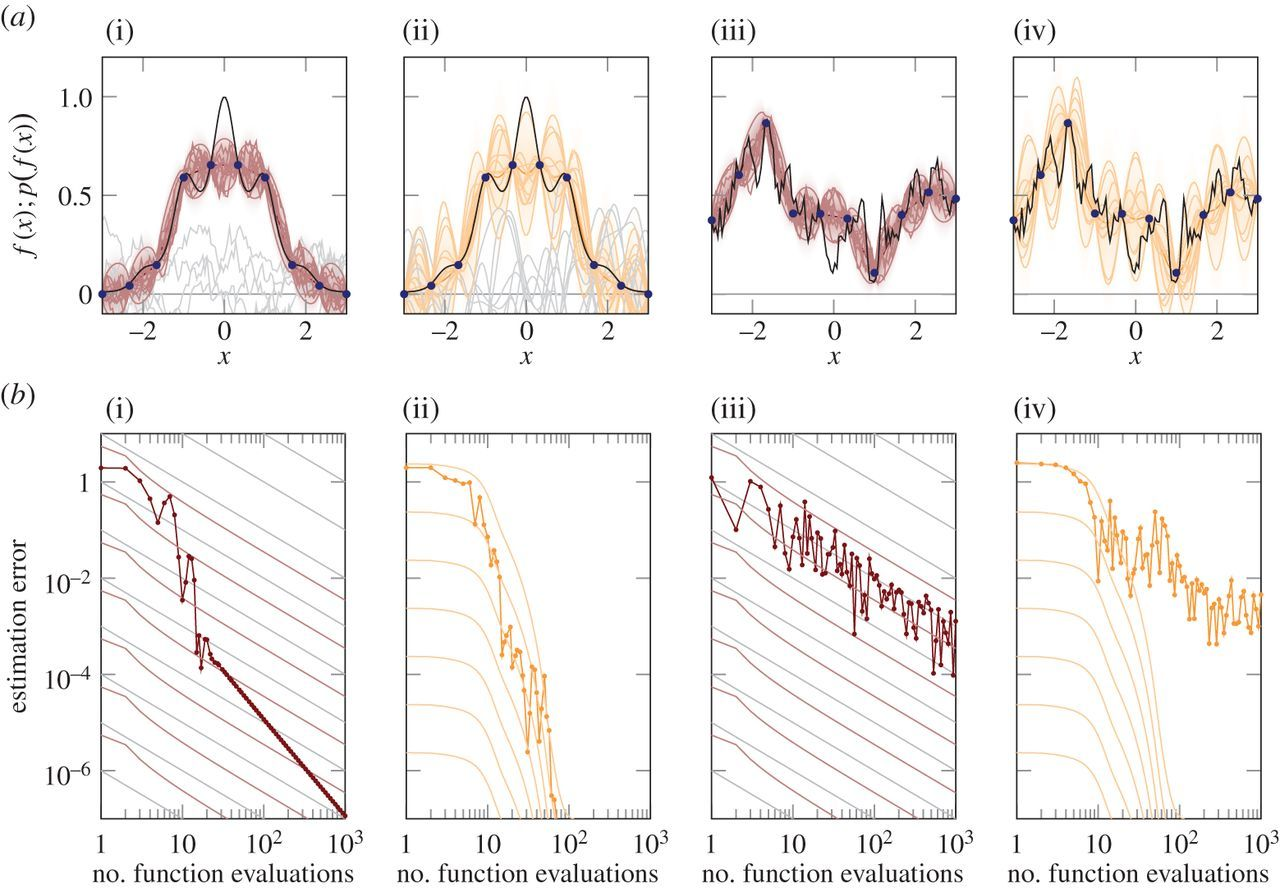
\includegraphics[width=0.45\textwidth]{rspa20150142f01.jpg}
%         % \caption{Integration with different kernel functions}
%         \label{f: quad_bayes}
%     \end{figure}
        
%     % (\textbf{follow up works treat probabilistic models as state estimation problems})

%     \item GP Learning for noisy state data \cite{ye_gaussian_2023}
% \end{enumerate}

% \end{frame}

% % \begin{frame}{Notation}


% % \end{frame}

% \section{Methodology}
% \begin{frame}{Methodology I}

% Model uncertainty jointly for time derivative and solution $(u_t, u)$

% \textbf{Prior Model: }
% $$\left.\begin{bmatrix}u_t(\mathbf{t_j})\\u(\mathbf{t_k})\end{bmatrix}\sim\mathcal{GP}\left(\begin{bmatrix}m_t^0(\mathbf{t_j})\\m^0(\mathbf{t_k})\end{bmatrix}\right.,\begin{bmatrix}C_t^0(\mathbf{t_j},\mathbf{t_j})&\int_0^{\mathbf{t_k}}C_t^0(\mathbf{t_j},\mathbf{z})\mathrm{d}\mathbf{z}\\\int_0^{\mathbf{t_k}}C_t^0(\mathbf{z},\mathbf{t_j})\mathrm{d}\mathbf{z}&C^0(\mathbf{t_k},\mathbf{t_k})\end{bmatrix}\right)$$

% \textbf{Covariance Operators:}

% $R_\lambda (t_j, t_k) = \exp (-(t_j - t_k)^2)/2\lambda^2$

% $R_\lambda (t_j, t_k) = \mathbf{1}_{(t_j - \lambda, t_j + \lambda)}(t_k)$ - for models with second derivative discontinuities.

% $Q_\lambda (t_j, t_k) = \int_{0}^{t_j}R_\lambda (z, t_k) dz$

% Convolve operators with themselves for prior covariance.

% \end{frame}

% \begin{frame}{Covariances}

% $$\begin{aligned}C_t^0(t_j,t_k)=\alpha^{-1}\int_{\mathbb{R}}R_\lambda(t_j,z)R_\lambda(t_k,z)\mathrm{d}z,\end{aligned}$$

% $$C^0(t_j,t_k)=\alpha^{-1}\intop_{\mathbb{R}}Q_\lambda(t_j,z)Q_\lambda(t_k,z)\mathrm{d}z$$

% Parameters: Lengthscale $\lambda$, Prior precision $\alpha$

% \end{frame}

% \begin{frame}{Constraints}

% The means should be related as follows for all times:
    
%     $$\int m_t^0 (z) dz = m^0(t)$$

% Enforce the initial condition i.e.  $u(0)=u_0=m^0(0)$ (this is ensured by the previous convolutions! - since $C^0(0, 0)=0$) (see supplementary material for closed form expressions - \url{https://www.doi.org/10.1214/16-BA1017SUPP})

% Analogously define the cross covariance terms:

% $$\begin{aligned}\int_0^{t_j}C_t^0(z,t_k)\mathrm{d}z~=~\alpha^{-1}\int_{\mathbb{R}}Q_\lambda(t_j,z)R_\lambda(t_k,z)\mathrm{d}z\end{aligned}$$

% \end{frame}


% \begin{frame}{Methodology II}
% \textbf{Sequence of updates: }

% \textbf{First Update:}
% $s=(s_1, \cdots, s_N)$ - pre-discretized grid in time for model updates

% $s_1$ = 0 i.e. evaluate RHS for known IC!

% $f_1 \equiv f(s_1, u^{\ast}(s_1), \theta) = u_t^{\ast}(s_1)$

% Condition on $f_1$ to update the prior GP:
% $$\left [ \begin{bmatrix}u_t(\mathbf{t_j})\\u(\mathbf{t_k})\end{bmatrix} \vert f_1 \right ]\sim\mathcal{GP}\left (\begin{bmatrix}m_t^1(\mathbf{t_j})\\m^1(\mathbf{t_k})\end{bmatrix},\begin{bmatrix}C_t^1(\mathbf{t_j},\mathbf{t_j})&\int_0^{\mathbf{t_k}}C_t^1(\mathbf{t_j},\mathbf{z})\mathrm{dz}\\ \int_0^{\mathbf{t_k}}C_t^1(\mathbf{z},\mathbf{t_j})\mathrm{dz}&C^1(\mathbf{t_k},\mathbf{t_k})\end{bmatrix} \right )$$

% \end{frame}

% \begin{frame}{Mean and covariance expressions}
%     $$\begin{gathered}
%         m_t^1(\mathbf{t_j}) =m_t^0(\mathbf{t_j})+C_t^0(\mathbf{t_j},s_1)C_t^0(s_1,s_1)^{-1}\textcolor{red}{\left\{\text{f}_1-m_t^0(s_1)\right\}}, \\
%         m^1(\mathbf{t_k}) =m^0(\mathbf{t_k})+C_t^0(s_1,s_1)^{-1}\intop_0^\mathbf{t_k}C_t^0(\mathbf{z},s_1)\mathrm{d}\mathbf{z}\textcolor{red}{\left\{\mathrm{f}_1-m_t^0(s_1)\right\}}, 
%         \end{gathered}$$

%         $$\begin{aligned}
%             C_t^1(\mathbf{t_j},\mathbf{t_j})& =C_t^0(\mathbf{t_j},\mathbf{t_j})-C_t^0(\mathbf{t_j},s_1)C_t^0(s_1,s_1)^{-1}C_t^0(s_1,\mathbf{t_j}),  \\
%             C^1(\mathbf{t_k},\mathbf{t_k})& =C^0(\mathbf{t_k},\mathbf{t_k})-\left\{\intop_0^{t_k} C_t^0(\mathbf{z},s_1)\mathrm{d}\mathbf{z}\right\}C_t^0(s_1,s_1)^{-1}\\\left \{\int_0^{t_k}C_t^0(\mathbf{z},s_1)\mathrm{d}\mathbf{z}\right \}
%         \end{aligned}$$
    
% \end{frame}

% \begin{frame}{Updates at unknown $f$}
% Draw multiple samples of state at next timestep from $m^1$ and $C^1$:

% $$u(s_2) \sim \mathcal{N}(m^1(s_2), C^1(s_2))$$

% Get derivative at $s_2$ from known dynamics:
% $$f_2 \equiv f(s_2, u_1(s_2), \theta)$$

% Unknown PDF for $f_2$ in absence of exact solution!

% \textbf{Assumption: } Discrepancy decreases with decreasing uncertainty in value of $u(s_2)$, Gaussian error model:

% $$f_2 | u_t, f_1 \sim \mathcal{N}(u_t(s_2), \textcolor{red}{C_t^1(s_2, s_2)=r_1(s_2)})$$


% \end{frame}

% \begin{frame}{Methodology III}

% Updated GP:

% $\left [ \begin{bmatrix}u_t(\mathbf{t_j})\\u(\mathbf{t_k})\end{bmatrix} \bigg{\vert} f_2, f_1 \right ]\sim\mathcal{GP}\left (\begin{bmatrix}m_t^2(\mathbf{t_j})\\m^2(\mathbf{t_k})\end{bmatrix},\begin{bmatrix}C_t^2(\mathbf{t_j},\mathbf{t_j})&\int_0^{\mathbf{t_k}}C_t^2(\mathbf{t_j},\mathbf{z})\mathrm{dz}\\ \int_0^{\mathbf{t_k}}C_t^2(\mathbf{z},\mathbf{t_j})\mathrm{dz}&C^2(\mathbf{t_k},\mathbf{t_k})\end{bmatrix} \right )$


% Repeat steps up to $s_N$, final output: Posterior probability distribution $[u_t, u | f]$

% \textbf{Key Result: } For $r_n(s)=0$ i.e. no uncertainty in estimation of $f_{2, \cdots, N}$ the GP converges in $L^1$ to exact solution as the grid is refined:

% $$\begin{aligned}\operatorname{E}\left(|u(t)-u^*(t)|\mid N\right)&=O(h),\quad\mathrm{~as~}\alpha^{-1},\lambda\to0\end{aligned}$$

% \end{frame}


% \begin{frame}{Methodology IV}
% \textbf{Hyperparameter updates:}
% Observe states through noisy measurements described by action of operator $H$, infer hyperparameters through MCMC (Algorithm 2 of paper)
% % $$\begin{array}{rcl}\left[\mathbf{y}\mid\mathbf{u},\theta,\Sigma\right]&\propto&\rho\left\{\mathbf{y}-H\left(\mathbf{u},\theta\right)\right\},\\[\mathbf{u}\mid\theta,\Psi,N]&=&p\left(\mathbf{u}\mid\theta,\Psi,N\right),\\[\theta,\Psi,\Sigma]&=&\pi(\theta,\Psi,\Sigma),\end{array}$$

% \end{frame}

% \section{Key Results, Paper II}
% \begin{frame}{Results I}
%     Provide quantified discretization uncertainty for nonlinear delay system - suggestion is that lack of model fit to measurements means model discrepancy must be addressed.

%     \begin{figure}
%         \centering
%         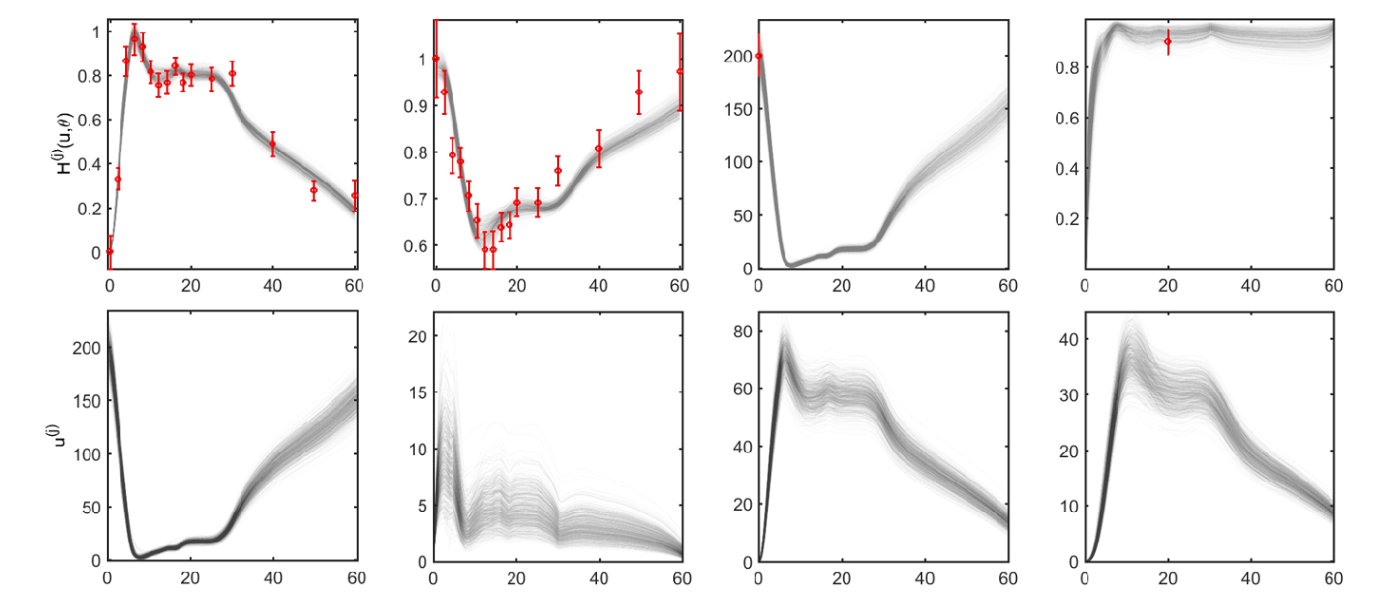
\includegraphics[width=0.8\textwidth]{disc_uc.png}
%         % \caption{Integration with different kernel functions}
%         \label{f: disc_uc}
%     \end{figure}


%     (show other results from paper)
% \end{frame}

% \begin{frame}{TLDR for Paper II}
% Link: \cite{ye_gaussian_2023}
% Similar ideas for problem setup (except specification of mean function, and no updating of GP over multiple timesteps - direct fit to observed data)!
% $$\left.\begin{bmatrix}x_i(t)\\\dot{x}_i(t)\end{bmatrix}\sim\text{vec-}\mathcal{GP}\left(\begin{bmatrix}0\\0\end{bmatrix}\right.,\begin{bmatrix}\kappa_i(t,t^{\prime})&\partial_{t^{\prime}}\kappa_i(t,t^{\prime})\\\partial_t\kappa_i(t,t^{\prime})&\partial_t\partial_{t^{\prime}}\kappa_i(t,t^{\prime})\end{bmatrix}\right)$$


% Joint normal distribution on states $u_i$ and derivatives $d_i$:
% $p\left(\mathbf{d}_{i}=f_{i}(\mathbf{U};\boldsymbol{\theta}_{i}),\mathbf{u}_{i}|\boldsymbol{\theta}_{i}\right)\propto\exp \left ( -\frac12\begin{bmatrix}f_{i}(\mathbf{U};\boldsymbol{\theta}_{i})\\\mathbf{u}_{i}\end{bmatrix}.^{\mathsf{T}}\begin{bmatrix}\mathbf{K}_{i}^{dd}&\mathbf{K}_{i}^{du}\\\mathbf{K}_{i}^{ud}&\mathbf{K}_{i}^{uu}\end{bmatrix}^{-1}\begin{bmatrix}f_{i}(\mathbf{U};\boldsymbol{\theta}_{i})\\\mathbf{u}_{i}\end{bmatrix} \right )$
% \end{frame}

% \begin{frame}{TLDR for Paper II}
%     Fit data points to GP described by above, and get posterior update for $\theta$:

%     $\begin{gathered}p\left(\boldsymbol{\theta}_i|\mathbf{d}_i=f_i(\mathbf{U};\boldsymbol{\theta}_i),\mathbf{u}_i\right)\propto p\left(\mathbf{d}_i=f_i(\mathbf{U};\boldsymbol{\theta}_i),\mathbf{u}_i|\left.\boldsymbol{\theta}_i\right)p(\boldsymbol{\theta}_i)\right.\\\propto \exp\left(-\frac12\left(f_i(\mathbf{U};\boldsymbol{\theta}_i)^\mathsf{T}\mathbf{R}_i^{dd}f_i(\mathbf{U};\boldsymbol{\theta}_i)+2f_i(\mathbf{U};\boldsymbol{\theta}_i)^\mathsf{T}\mathbf{R}_i^{du}\mathbf{u}_i+\|\boldsymbol{\theta}_i\|_{\boldsymbol{\Lambda}_i}^2\right)\right)\end{gathered}$
    
% \end{frame}


% \begin{frame}{Results II}
    
% Results provided for extrapolation of trajectories given noisy data (cases of known parametrization and parametrization approximated by shallow NN)

% \begin{figure}
%     \centering
%     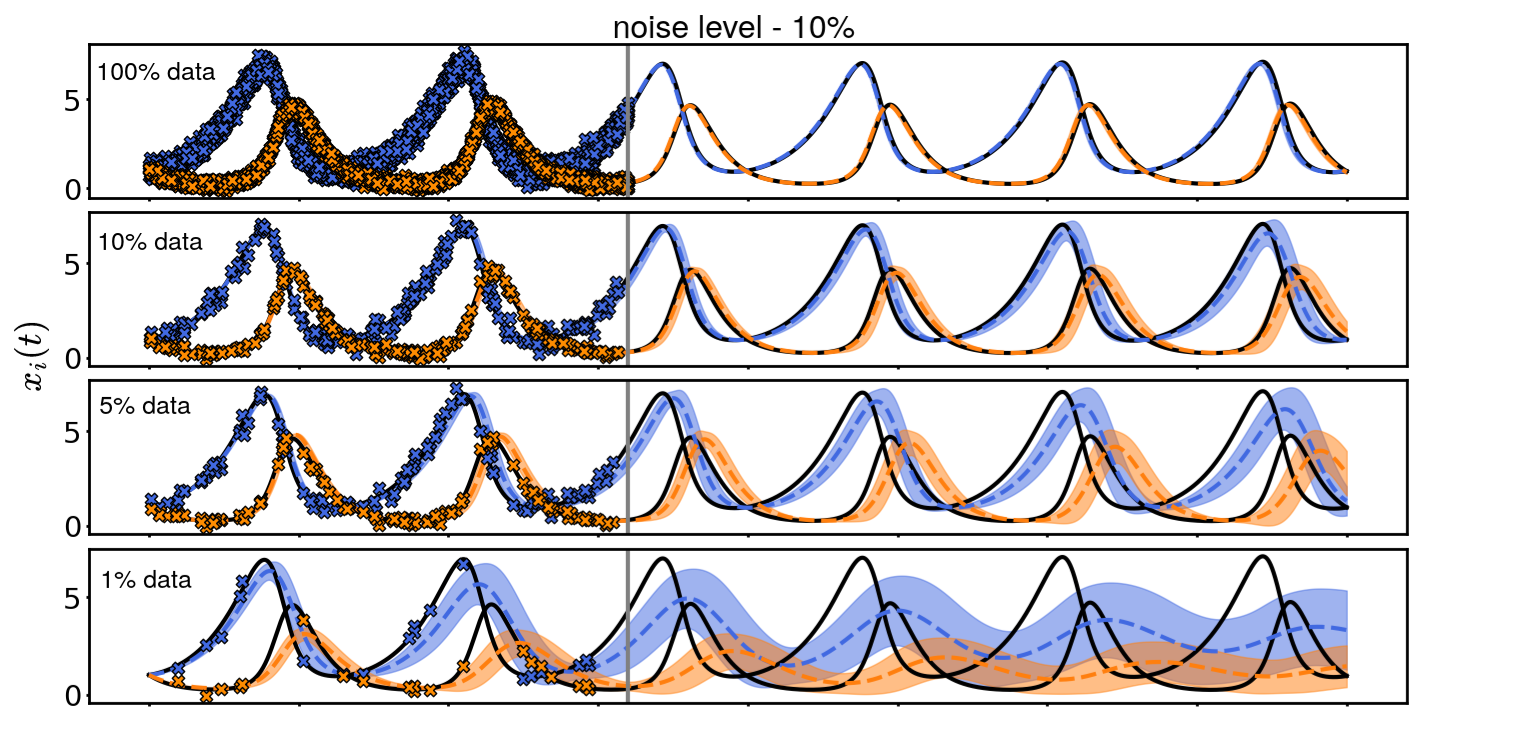
\includegraphics[width=0.8\textwidth]{noisy_data_reconstruction.png}
%     % \caption{Integration with different kernel functions}
%     \label{f: noisy_uc}
% \end{figure}
% \end{frame}


% \begin{frame}{TLDR for Paper III}
%     Gaussian Processes meet Neural ODEs (learning dynamics, model calibration etc.) - \url{https://doi.org/10.1098/rsta.2021.0201} \cite{bhouri_gaussian_2022}

%     Differences from Paper II:

% \end{frame}

% \begin{frame}{TLDR for Paper IV}
%     Latent Force Models \url{https://proceedings.mlr.press/v5/alvarez09a.html} \cite{pmlr-v5-alvarez09a}
% \end{frame}

% \begin{frame}{Summing up}
% \begin{itemize}
% \item GPs offer a convenient means to build probabilistic models for estimating states with numerical approximations / data-driven methods. (case of exact but unknown solution, not misspecified model in paper 1!) - however potential \emph{scalability issues} for large $N$ and large input size (paper II)

% \item The key assumptions lie in selection of kernel functions, error process for derivatives in subsequent updates - important to avoid physically inconsistent trajectories.

% \item Above schemes need to be extended to higher-order deterministic solvers, adaptive step-size solvers and so on - this falls neatly into the works for \textcolor{red}{\emph{probabilistic numerics!}}
% \end{itemize}
% \end{frame}


% \begin{frame}{Additional Resources:}
% \begin{enumerate}
%     \item Filtering Approach for ODEs: \url{https://probnum.readthedocs.io/en/latest/tutorials/odes/uncertainties_odefilters.html}
    
%     \item Code for Paper 1: \url{https://github.com/ochkrebtii/uqdes}
% \end{enumerate}
% \end{frame}


\begin{frame}[allowframebreaks]
    \frametitle{References}
    \bibliographystyle{chicago}
    \bibliography{myRef}
\end{frame}

% \section{Backup}
% \begin{frame}{}
% \begin{center}
%     \Large{Thank you!}
% \end{center}
        
% \end{frame}

% Nice 15 minute read on the subject and the philosophy: \url{https://www.stochasticlifestyle.com/how-to-train-interpretable-neural-networks-that-accurately-extrapolate-from-small-data/}

% \end{frame}
% \begin{frame}{Backup 5: Implementation}
% Some other day.
% \end{frame}
\end{document}
